\documentclass[12pt]{article}
\usepackage{amsmath}
\usepackage[round]{natbib}
%\usepackage{times}
\usepackage{graphicx}
%\usepackage{courier}
\usepackage{mathpazo}
\usepackage{mathrsfs}
\usepackage{bm}
\usepackage[colorlinks,linkcolor=red,anchorcolor=blue,citecolor=blue]{hyperref}
\usepackage[verbose,letterpaper,tmargin=1in,bmargin=.75in,lmargin=.75in,rmargin=1in]{geometry}
\usepackage{amsthm}
\usepackage{pdflscape}

\title{Bayesian Quantile Regression using a  Mixture of P\'{o}lya Tree Prior}
\date{\today}
\author{}

\newtheorem{thm}{Theorem}[section]
\newtheorem{deff}[thm]{Definition}
\newtheorem{rmk}[thm]{Remark}
\newtheorem{cor}[thm]{Corollary}
\newtheorem{emp}[thm]{Example}
\newtheorem{lem}[thm]{Lemma}
\newtheorem{pps}[thm]{Proposition}

\newcommand{\polya}{P\'{o}lya}
\newcommand{\iid}{\stackrel{\mbox{i.i.d}}{\sim}}
\DeclareMathOperator{\pr}{p}
\DeclareMathOperator{\pt}{PT}
\DeclareMathOperator{\LN}{LN}
\usepackage{booktabs}

\begin{document}
% \setlength\parindent{0pt}

\maketitle{}

\begin{abstract}
\end{abstract}

\section{Introduction}

Quantile regression is a powerful way of studying the relationship
between response and covariates when one (or several) quantiles are of
interest.  The dependence between upper or lower quantiles of the
response variable and the covariates are expected to vary
differentially relative to that of the average. This is often of
interest in econometrics, educational studies, biomedical studies, and
environment studies \citep{yu2001,buchinsky1994,
  buchinsky1998,he1998,koenker1999, wei2006, yu2003}.  A comprehensive
review of quantile regression was presented by \citet{koenker2005}.
Furthermore, mean regression provides less information about the
relationship of the average with linear combination of covariates;
quantile regression can offer a more complete description of the
conditional distribution of the response.

The traditional frequentist approach was proposed by
\citet{koenker1978} for a single quantile ($\tau$) with estimators
derived by minimizing a loss check function $\sum_{i=1}^n
\rho_{\tau}(y_i - \bm{x_i'\beta})$, where $\rho_{\tau}(\epsilon) =
\epsilon (\tau- \mathrm{I}(\epsilon < 0))$. They do not make any
distributional assumptions for residuals and use linear programming
techniques for estimation.  The popularity of this approach is due to
its computational efficiency, well-developed asymptotic properties,
and straightforward extensions to simultaneous quantile regression and
random effect models. However, asymptotic inference may not be
accurate for small sample sizes.

Bayesian approaches offer exact inference. Motivated by the loss check
function, \citet{yu2001} proposed an asymmetric Laplace distribution
for the error term, such that maximizing the posterior distribution is
equivalent to minimizing the check function. Other than parametric
Bayesian approaches, some semiparametric methods have been proposed
for median regression. \citet{walker1999} used a diffuse finite
\polya{} Tree prior for the error term. \citet{kottas2001} modeled the
error by two families of median zero distribution using a mixture
Dirichlet process priors, which is very useful for unimodal error
distributions. \citet{hanson2002} adopted mixture of \polya{} Tree
prior on error term to make inference in regression model. They
illustrated the implementation on AFT model for the median survival
time, which showed robustness of \polya{} in terms of multimodality
and skewness.  \citet{reich2010} uses an infinite mixture of Gaussian
densities on the residual.  Other recent approaches include quantile
pyramid priors, mixture of Dirichlet process priors of multivariate
normal distributions and infinite mixture of Gaussian densities which
put quantile constraints on the residuals \citep{hjort2007,hjort2009,
  kottas2009}.

Like the asymmetric Laplace distribution, all of the above methods are
single semiparametric quantile regression methods, which have some
limitations. The densities have their restrictive mode at the quantile
of interest, which is not appropriate when extreme quantiles are being
investigated. Other criticisms include crossed quantile lines,
monotonicity constraints and difficulty in making inference for
quantile regression parameter for an interval of $\tau$s. Joint
inference is poor in borrowing information through single quantile
regressions. It is not coherent to pool from every individual quantile
regression, because the sampling distribution of $Y$ for $\tau_1$ is
usually different from that under quantile $\tau_2$ since they are
assuming different error distribution under two different quantile
regressions \citep{tokdar2011}.

In order to solve those problems, simultaneous linear quantile
regression have been proposed by \citet{tokdar2011}.  Another popular
approach is to assign a nonparametric model for the error term to
avoid the monotonicity problem \citep{scaccia2003, geweke2007,
  taddy2010}.

We use a mixture of \polya{} Tree (PT) priors in our approach. PT
priors were introduced decades ago \citep{freedman1963, fabius1964,
  ferguson1974} and \citet{lavine1992, lavine1994} extended them to
\polya{} Tree models. The major advantage of \polya{} Tree over
Dirichlet process is that it can be absolutely continuous with
probability 1 and it can be easily tractable. In a regression context,
\citet{walker1997, walker1999} assigned a finite \polya{} Tree prior
to the random effects in a generalized linear mixed
model. \citet{berger2001} used a mixture of \polya{} Tree comparing
data distribution coming from parametric distribution or mixture of
\polya{} Tree. They used a \polya{} tree process to test the fit of
data to a parametric model by embedding the parametric model in a
nonparametric alternative and computing the Bayes factor of the
parametric model to the nonparametric alternative.  As mentioned
earlier \citet{hanson2002} modeled the error term as a mixture of
\polya{} tree prior in the regression model.

Multivariate regression is also possible with \polya{}
Trees. \citet{paddock1999, paddock2002} studied multivariate \polya{}
Tree in a k-dimensional hypercube. \citet{hanson2006} constructed a
general framework for multivariate random variable with a \polya{}
Tree distribution. \citet{jara2009} extended the multivariate mixture
of \polya{} Tree prior with a directional orthogonal matrix.  He also
demonstrated how to fit a generalized mixed effect model by modeling
multivariate random effects with multivariate mixture of \polya{} Tree
priors.

In this article, we present a Bayesian approach by adopting a mixture
of \polya{} Tree prior for the regression error term, and we account
for the change of quantile regression parameter via heterogeneity of
the error term. As a result, several quantile regression can be fit
simultaneously and there is a closed form for posterior quantile
regression parameter. Exact inference can be made through Monte Carlo
Markov Chain (MCMC) approach, and our method avoids the problem of
crossing quantile lines that occurs in the traditional frequentist
quantile regressions.

The rest of the paper is organized as follows. In
section~\ref{ch2:sec:model}, we introduce the heterogeneity model and
derive a closed form for marginalized posterior quantile regression
parameter with mixture of \polya{} tree prior.  In
section~\ref{ch2:sec:simulations}, we conduct some simulation studies and
apply our approach on a real data example in
section~\ref{ch2:sec:tours}. Finally, conclusions and discussions are
presented in section~\ref{ch2:sec:discussion}.

\section{Model, Priors, and Computations}
\label{ch2:sec:model}
\subsection{Heterogeneity Model}
Let $Y$ be a random variable with CDF $F$.  The $\tau$th quantile of
$Y$ is defined as
\begin{displaymath}
  Q_Y(\tau) = \underset{y}{\inf} \left\{ y: F(y) \ge \tau \right\}.
\end{displaymath}
If covariates $\bm{x_1, \ldots, x_n}$ are of interest, then the
quantile regression parameter satisfies the following condition:
\begin{displaymath}
  Q_Y(\tau) = \bm{X'\beta}(\tau),
\end{displaymath}
where $\bm{X}$ is the matrix of covariates including an intercept.  If
$F$ is continuous, then $F(\bm{X'\beta}(\tau)) = \tau$, i.e., $\pr(Y
\le \bm{X'\beta}(\tau)) = \tau$.

Now, consider a location shift model,
\begin{displaymath}
  y_i = \bm{x}_i\beta + \epsilon_i,
\end{displaymath}
where $\epsilon_i \stackrel{\mbox{i.i.d}}{\sim} F_{\epsilon}$. Then,
the $\tau$th quantile regression parameter can be expressed as
\begin{equation} \label{ch2:eq:reg} \bm{\beta}(\tau) = \bm{\beta} +
  F^{-1}_{\epsilon}(\tau) \bm{e}_1,
\end{equation}
where $\bm{e}_1 = [1, 0, \ldots, 0]^T$, and $F^{-1}_{\epsilon}(\tau)$
is the $\tau$th quantile for error $\epsilon$.

As we can see from equation~(\ref{ch2:eq:reg}), if the model is
homogeneous, i.e., i.i.d case, then for different quantiles $\tau$,
the corresponding quantile regression parameters only vary in the
first component, the intercept. The rest of the quantile regression
parameters stay the same. Therefore, quantile lines for different
quantiles are parallel to each other.

Now, consider the heterogeneous linear regression model from
\citet{he1998}
\begin{equation}\label{ch2:eq:he}
  y_i = \bm{x}_i'\bm{\beta} + (\bm{x}_i'\bm{\gamma}) \epsilon_i,
\end{equation}
where $\bm{x_i'\gamma}$ is positive for all $i$. Under this model, the
$\tau$th quantile regression parameter is
\begin{equation}\label{ch2:eq:quan}
  \bm{\beta}(\tau) = \bm{\beta} + F^{-1}_{\epsilon}(\tau) \bm{\gamma},
\end{equation}

Quantile lines are no longer parallel under the heterogeneous linear
model which adds considerably more flexibility in the model.

We use a mixture of \polya{} Tree prior for the error term in equation~(\ref{ch2:eq:he})
 and derive a closed form for posterior quantile
regression parameter in~(\ref{ch2:eq:quan}).  Since \polya{} tree is a
very flexible way to model the unknown distribution, our approach
makes fewer assumptions.  Exact inference can be made through MCMC using
functionals of posterior samples. The next subsection briefly reviews
the \polya{} tree priors and their relevant properties.

\subsection{\polya{} Tree}
\citet{lavine1992, lavine1994} and \citet{mauldin1992} developed
theory for \polya{} tress priors as a generalization of the Dirichlet
process \citep{ferguson1974}. Denote $E=\{0,1\}$ and $E^m$ as the
m-fold product of $E$, $E^0= \emptyset$, $E^{*} = \cup_0^{\infty} E^m$
and $\Omega$ be a separable measurable space, $\pi_0 = \Omega$, $\Pi=
\{ \pi_m: m=0,1, \ldots \} $ be a separating binary tree of partitions
of $\Omega$. In addition, define $B_{\emptyset} = \Omega$ and $\forall
\epsilon=\epsilon_1\cdots \epsilon_m \in E^{*}$, $B_{\epsilon 0}$ and
$B_{\epsilon 1}$ are the two partition of $B_{\epsilon}$.
\begin{deff}
  A random probability measure $G$ on $(\Omega, \mathcal{F})$ is said
  to have a \polya{} tree distribution, or a \polya{} tree prior with
  parameter $(\Pi, \mathcal{A})$, written as $G|\Pi, \mathcal{A} \sim
  \pt (\Pi, \mathcal{A})$, if there exist nonnegative numbers
  $\mathcal{A}= \left\{ \alpha_{\epsilon}, \epsilon \in E^{*}
  \right\}$ and random vectors $\mathcal{Y} = \left\{ Y_{\epsilon} :
    \epsilon \in E^{*} \right\}$ such that the following hold:
  \begin{enumerate}
  \item\label{ch2:item:1} all the random variables in $\mathcal{Y}$ are
    independent;
  \item $Y_{\epsilon}= (Y_{\epsilon 0}, Y_{\epsilon 1}) \sim
    \mathrm{Dirichlet}(\alpha_{\epsilon 0 }, \alpha_{\epsilon 1}),
    \forall \epsilon \in E^{*}$;
  \item $\forall m=1,2, \ldots$, and $\forall \epsilon \in E^{*},
    G(B_{\epsilon_{1}, \ldots, \epsilon_m}) = \prod_{j=1}^m
    Y_{\epsilon_1 \cdots \epsilon_j}$.
  \end{enumerate}
\end{deff}

\subsubsection{\polya{} Tree Parameters}
There are two parameters in the \polya{} tree distribution $(\Pi,
\mathcal{A})$. A \polya{} tree is centered around a
  pre-specified distribution $G_0$, which is called the baseline
  measure. The $\mathcal{A}$ family determines how much $G$ can
deviate from $G_0$. \citet{ferguson1974} pointed out $\alpha_{\epsilon} = 1
$ yields a $G$ that is absolutely continuous with probability 1, and
$\alpha_{\epsilon_1, \ldots, \epsilon_m} = m^2$ yields $G$ that is
absolutely continuous with probability 1. \citet{walker1999} and
\citet{paddock1999} considered $\alpha_{\epsilon_1, \ldots,
  \epsilon_m} = cm^2$, where $c > 0$. \citet{berger2001} considered
$\alpha_{\epsilon_1, \ldots, \epsilon_m} = c \rho(m)$. In general, any
$\rho(m) $ such that $\sum_{m=1}^{\infty} \rho(m)^{-1} < \infty$
guarantees $G$ to be absolutely continuous. In our case, we adopt
$\alpha_{\epsilon_1, \ldots, \epsilon_m} = cm^2$.

As to the partition parameter $\Pi$, the canonical way of constructing
a \polya{} tree distribution $G$ centering on $G_0$, a continuous CDF
is to choose $B_0 = G^{-1}_0 ([0, 1/2]), B_1 = G^{-1}_0 ((1/2,1])$,
such that $G(B_0) = G(B_1)= 1/2$. Furthermore, for all $\epsilon \in
E^{*}$, choose $B_{\epsilon 0 }$ and $B_{\epsilon 1}$ to satisfy
$G(B_{\epsilon 0 } |B_{\epsilon} ) = G(B_{\epsilon 1} | B_{\epsilon})
= 1/2 $, then any choice of $\mathcal{A} $ makes $G$ coincide with
$G_0$. A simple example is to choose $B_{\epsilon 0} $ and
$B_{\epsilon 1}$ in level $m$ by setting them as $G^{-1}_0 \left(
  (k/2^m, (k+1)/2^m] \right)$, for $k=0, \ldots, 2^m-1$.

\subsubsection{Some properties of \polya{} Tree}
Suppose $G \sim \pt (\Pi, \mathcal{A})$ is a random probability
measure and $\epsilon_1, \epsilon_2, \ldots$ are random samples from
$G$.

\begin{deff}[Expectation of \polya{} Tree]
  $F= E(G)$ as a probability measure is defined by $F(B) = E(G(B)),
  \forall B \in \mathcal{B}$. By the definition of \polya{} tree, for
  any $\epsilon \in E^{*}$,
  \begin{displaymath}
    F(B_{\epsilon})  = E(G(B_{\epsilon})) = \prod_{j=1}^m
    \frac{\alpha_{\epsilon_1, \ldots, \epsilon_j}}{\alpha_{\epsilon_1,
        \ldots, \epsilon_{j-1},0} + \alpha_{\epsilon_1, \ldots, \epsilon_{j-1},1}}.
  \end{displaymath}
\end{deff}

\begin{rmk}
  If $G$ is constructed based on baseline measure $G_0$ and we set
  $\alpha_{\epsilon_1, \ldots, \epsilon_m} = cm^2 $,
  $\alpha_{\epsilon_0 }= \alpha_{\epsilon_1}$, then $\forall B \in
  \mathcal{B}, F(B) = G_0(B)$; thus, $F=G_0$, if there is no data.
\end{rmk}

\begin{deff}[Density Function]
  Suppose $F=E(G), G|\Pi, \mathcal{A} \sim \pt (\Pi, \mathcal{A})$,
  where $G_0 $ is the baseline measure. Then, using the canonical
  construction, $F=G_0$ (as shown above), the density function is
  \begin{equation}\label{ch2:eq:density}
    f(y) = \left[ \prod_{j=1}^m \frac{ \alpha_{\epsilon_1, \ldots,
          \epsilon_j}(y)}{\alpha_{\epsilon_1, \ldots, \epsilon_{j-1},0}(y)
        + \alpha_{\epsilon_1, \ldots, \epsilon_{j-1},1}(y)} \right] 2^{m } g_0(y),
  \end{equation}
  where $g_0$ is the pdf of $G_0$.
\end{deff}

\begin{rmk}
  When using the canonical construction with no data,
  $\alpha_{\epsilon_0 } = \alpha_{\epsilon_1}$, equation~(\ref{ch2:eq:density})
  simplifies to
  \begin{displaymath}
    f(y) = g_0(y).
  \end{displaymath}
\end{rmk}

\begin{rmk}[Conjugacy] If $y_1, \ldots, y_n | G \sim G, G|\Pi,
  \mathcal{A} \sim \pt (\Pi, \mathcal{A})$, then $G|y_1, \ldots, y_n,
  \Pi, \mathcal{A} \sim \pt (\Pi, \mathcal{A}^{*})$, where in
  $\mathcal{A}^{*}, \forall \epsilon \in E^{*}$,
  \begin{displaymath}
    \alpha_{\epsilon}^{*} = \alpha_{\epsilon} + n_{\epsilon}(y_1, \ldots, y_n),
  \end{displaymath}
  where $n_{\epsilon}(y_1, \ldots, y_n)$ indicates the count of how many
  samples of $y_1, \ldots, y_n$ fall in $B_{\epsilon}$.
\end{rmk}

\subsubsection{Mixture of \polya{} Trees}
The behavior of a single \polya{} tree highly depends on how the
partition is specified. A random probability measure $G_\theta$ is
said to be a mixture of \polya{} tree if there exists a random
variable $\theta$ with distribution $h_{\theta}$, and \polya{} tree
parameters $(\Pi^{\theta}, \mathcal{A}^{\theta})$ such that
$G_{\theta} | \theta=\theta \sim \pt (\Pi^{\theta},
\mathcal{A}^{\theta})$.

\begin{emp}
  Suppose $G_0 = \mathrm{N}(\mu, \sigma^2)$ is the baseline measure.
  For $\epsilon \in E^{*}, \alpha_{\epsilon_m} = cm^2 $, $\bm{\theta}=
  (\mu, \sigma, c)$ is the mixing index and the distribution on
  $\Theta = (\mu, \sigma, c) $ is the mixing distribution.
\end{emp}
With the mixture of \polya{} tree, the influence of the partition is
lessened. Thus, inference will not be affected greatly by a single
\polya{} tree distribution.

\subsubsection{Predictive Error Density, Cumulative Density Function
  and Quantiles}
Suppose $G_{\theta}$ is the baseline
measure, $g_0(y)$ is the density
function. $\Pi^{\theta}$ is defined as
\begin{displaymath}
  B^{\theta}_{\epsilon_1, \ldots, \epsilon_m} = \left( G^{-1}_{\theta}
    \left( \frac{k}{2^m} \right), G^{-1}_{\theta}\left( \frac{k+1}{2^m} \right) \right),
\end{displaymath}
where $k$ is the index of partition $\epsilon_1, \ldots, \epsilon_m$
in level $m$. $\mathcal{A}^c$ is defined as
\begin{displaymath}
  \alpha_{\epsilon_1, \ldots, \epsilon_m} = cm^2.
\end{displaymath}
Therefore, the error model is
\begin{align*}
  y_1, \ldots, y_n |G_{\theta} & \iid G, \\
  G|\Pi^{\theta}, \mathcal{A}^{c} & \sim \pt (\Pi^{\theta},
  \mathcal{A}^{c}).
\end{align*}

The predictive density function of $Y|y_1, \ldots, y_n, \theta$,
marginalizing out $G$, is
\begin{equation}
  \label{ch2:eq:pred}
  f_Y^{\theta} (y|y_1, \ldots, y_n)  = \lim_{m \to \infty} \left(
    \prod_{j=2}^m \frac{cj^2 + n_{\epsilon_1 \cdots \epsilon_j(x) }(y_1, \ldots, y_n)}{2cj^2
      + n_{\epsilon_1 \cdots \epsilon_{j-1}(x)}(y_1, \ldots, y_n)}
  \right)2^{m-1} g_0(y),
\end{equation}
where $n_{\epsilon_1 \cdots \epsilon_j(x) }(y_1, \ldots, y_n)$
denotes the number of observations $y_1, \ldots, y_n$ dropping in the
bin $\epsilon_1 \cdots \epsilon_j$ where $y$ stays in the level
$j$. Notice that, if we restrict the first level weight as
$\alpha_0=\alpha_1=1$, then we only need to update levels beyond
the first level.

\begin{rmk}[The predictive density for Finite \polya{} Tree]
  In practice, a finite $M$ level \polya{} Tree is usually adopted to
  approximate the full \polya{} tree, in which, only up to $M$ levels
  are updated. The corresponding predictive density becomes
  \begin{equation}
    \label{ch2:eq:predf}
    f_Y^{\theta, M} (y|y_1, \ldots, y_n)  =  \left(
      \prod_{j=2}^M \frac{cj^2 + n_{\epsilon_1 \cdots \epsilon_j(x) }(y_1, \ldots, y_n)}{2cj^2
        + n_{\epsilon_1 \cdots \epsilon_{j-1}(x)}(y_1, \ldots, y_n)}
    \right)2^{M-1} g_0(y).
  \end{equation}
  The rule of thumb for choosing $M$ is to set $M=\log_2n$, where $n$
  is the sample size \citep{hanson2002}.
\end{rmk}

\citet{hanson2002} showed the approximation to (\ref{ch2:eq:pred}) given
in~(\ref{ch2:eq:predf}) is exact for $M$ large enough.  We now derive the
predictive cdf and the predictive quantile(s).

\begin{thm}
  Based on the predictive density function~(\ref{ch2:eq:predf}) of a
  finite \polya{} tree distribution, the predictive cumulative density
  function is
  \begin{equation}
    \label{ch2:eq:cdf}
    F^{\theta,M}_Y(y|y_1, \ldots, y_n) = \sum_{i=1}^{N-1} P_{i} + P_N
    \left( G_{\theta}(y)2^M -(N-1) \right),
  \end{equation}
  where
  \begin{align*}
    P_i &= \frac{1}{2} \left(\prod_{j=2}^M \frac{cj^2 + n_{j,\lceil
          i2^{j-M} \rceil}(y_1, \ldots, y_n)}{2cj^2 + n_{j-1,\lceil
          i2^{j-1-M} \rceil}(y_{1 },\ldots, y_n)} \right) \mbox{ and}\\
    N & = \left[ 2^{M } G_{\theta}(y) +1\right],
  \end{align*}
  in which $n_{j,\lceil i2^{j-M} \rceil}(y_1, \ldots, y_n)$ denotes
  the number of observations $y_1, \ldots, y_n$ in the $\lceil
  i2^{j-M} \rceil$ slot at level $j$, $\lceil \cdot \rceil$ is the
  ceiling function, and $[ \cdot ]$ is the floor function.
\end{thm}

\begin{proof}
  \begin{align*}
    F^{\theta,M}_Y(y| y_1, \ldots, y_n) & = \int_{-\infty}^y
    f_Y^{\theta,M} (y|y_1, \ldots, y_n) dx \\
    & = \int_{-\infty}^y \left( \prod_{j=2}^M \frac{cj^2 +
        n_{\epsilon_1 \cdots \epsilon_j(y) }(y_1, \ldots, y_n)}{2cj^2
        + n_{\epsilon_1 \cdots \epsilon_{j-1}(y)}(y_1, \ldots, y_n)}
    \right)2^{M-1} g_\theta(y) dy \\
    & = \sum_{i=1}^{N-1} \left( \prod_{j=2}^M \frac{cj^2 + n_{j,
          \lceil i2^{j-M} \rceil}(y_1, \ldots, y_n)}{2cj^2 + n_{j-1,
          \lceil i2^{j-1-M} \rceil}(y_1, \ldots, y_n)} 2^{M-1}
      \int_{\epsilon_{M,i}} g_{\theta}(y) dy \right) \\
    &+ \int_{G^{-1}_{\theta}((N-1)/2^M)}^y \left( \prod_{j=2}^M
      \frac{cj^2 + n_{j, \lceil N2^{j-M} \rceil}(y_1, \ldots,
        y_n)}{2cj^2 + n_{j-1, \lceil N2^{j-1-M} \rceil}(y_1, \ldots,
        y_n)}\right) 2^{M-1}
    g_{\theta}(y) dy \\
    & = \sum_{i=1}^{N-1} P_i + P_N 2^M \left( G_{\theta}(y) -
      G_{\theta}(G_{\theta}^{-1}\left( \frac{N-1}{2^M} \right)\right)\\
    & = \sum_{i=1}^{N-1}P_i + P_N \left( G_{\theta}(y) 2^M - (N-1)
    \right),
  \end{align*}
  where $\epsilon_{M,i}$ is the $i$th partition in level $M$.
\end{proof}

\begin{thm}
  The posterior predictive quantile of finite \polya{} tree
  distribution is
  \begin{equation}
    \label{ch2:eq:postquan}
    Q^{\theta, M}_{Y|y_1, \ldots, y_n}(\tau) = G^{-1}_{\theta} \left(
      \frac{\tau- \sum_{i=1}^N P_i + N P_N}{2^M P_N} \right),
  \end{equation}
  where $N$ satisfies $ \sum_{i=1}^{N-1} P_i < \tau \le \sum_{i=1}^N
  P_i$.
\end{thm}

\begin{proof}
  From equation~(\ref{ch2:eq:cdf}),
  \begin{align*}
    \tau = F^{\theta,M}_Y(y|y_1, \ldots, y_n) &= \sum_{i=1}^{N-1}
    P_{i} + P_N
    \left( G_{\theta}(y)2^M -(N-1) \right) \\
    \Rightarrow G_{\theta}(y) &= \frac{\tau - \sum_{i=1}^NP_i +
      NP_N}{2^MP_N} \\
    y & = G_{\theta}^{-1} \left(\frac{\tau - \sum_{i=1}^NP_i +
        NP_N}{2^MP_N} \right).
  \end{align*}
\end{proof}
Now the explicit form for quantile regression coefficients in equation~(\ref{ch2:eq:quan}) becomes:
\begin{equation}
  \label{ch2:eq:newquan}
  \bm{\beta}(\tau) = \bm{\beta} + \bm{\gamma}G_{\theta}^{-1}
  \left(\frac{\tau - \sum_{i=1}^NP_i +
      NP_N}{2^MP_N}  \right),
\end{equation}
where $P_i$ and $N$ are the notations in equation~(\ref{ch2:eq:cdf}) and
(\ref{ch2:eq:postquan}). This will greatly facilitate computations.

\subsection{Fully Bayesian Quantile Regression Specification with
  Mixture of \polya{} Tree Priors}
The full Bayesian specification of quantile regression is given as
follows,
\begin{align*}
  y_i& = \bm{x_i'\beta} + (\bm{x_i'\gamma}) \epsilon_{i}, i = 1,
  \ldots,
  n \\
  \epsilon_i |G_{\theta} & \iid G_{\theta} \\
  G_{\theta}|\Pi^{\theta}, \mathcal{A}^{\theta} & \sim \pt
  (\Pi^{\theta}, \mathcal{A}^{\theta}) \\
  \bm{\theta} = (\sigma, c) & \sim \pi_{\bm \theta}(\bm \theta) \\
  \bm{\beta} & \sim \pi_{\bm \beta}(\bm \beta)\\
  \bm{\gamma} &\sim \pi_{\bm \gamma}(\bm \gamma).
\end{align*}
In order to not confound the location parameter, $\epsilon_i $ or $G$
is set to have median 0 by fixing $\alpha_0=\alpha_1 = 1$. For the
similar reason, the first component of $\bm{\gamma}$ is fixed at 1.

The posterior distribution of $(\bm{\beta}, \bm{\gamma}, \sigma, c)$
is given as
\begin{equation}\label{ch2:eq:post}
  \begin{aligned}
    \pr(\bm{\beta}, \bm{\gamma}, \sigma, c|\bm{Y}) & \propto L(\bm{Y}|
    \bm{\beta}, \bm{\gamma}, \sigma, c) \pi_{\beta}(\beta)
    \pi_{\gamma}(\gamma) \pi_{\sigma}(\sigma) \pi_c(c) \\
    & = \frac{1}{\prod_{i=1}^n (\bm{x_i'\gamma})} \pr \left(
      \epsilon_1, \ldots, \epsilon_n | \bm{\beta}, \bm{\gamma},
      \sigma, c\right) \pi_{\beta}(\beta)
    \pi_{\gamma}(\gamma) \pi_{\sigma}(\sigma) \pi_c(c) \\
    & = \frac{1}{\prod_{i=1}^n (\bm{x_i'\gamma})} \pr
    \left(\epsilon_n| \epsilon_1, \ldots, \epsilon_{n-1}, \bm{\beta},
      \bm{\gamma}, \sigma, c\right) \cdots \pr \left(\epsilon_2|
      \epsilon_1, \bm{\beta}, \bm{\gamma}, \sigma, c\right) \pr
    \left(\epsilon_1| \bm{\beta}, \bm{\gamma},
      \sigma, c\right)\\
    & \qquad \pi_{\bm{\beta}}(\bm{\beta})
    \pi_{\bm{\gamma}}(\bm{\gamma}) \pi_{\sigma}(\sigma) \pi_c(c),
  \end{aligned}
\end{equation}
where $\epsilon_i = (y_i - \bm{x_i'\beta})/(\bm{x_i'\gamma})$.

For priors of $\sigma$ and $c$, we use diffuse gamma distributions,
\begin{align*}
  \pi(\sigma) & \sim \Gamma (1/2, 1/2), \\
  \pi(c) & \sim \Gamma(1/2, 1/2).
\end{align*}
Priors for the parameters $(\bm{\beta}, \bm{\gamma})$ are diffuse
p-dimensional normal distributions.  Spike priors on ($\bm \beta,
\bm \gamma$) are an alternative to do variable selection on both
quantile regression parameters and heterogeneity parameters and
improve efficiency.

Here we put continuous spike and slab priors on $(\bm \beta, \bm
\gamma)$ to shrink them toward zero for each component. The prior for
$j^{th}$ component of $\bm \beta$ and $\bm \gamma$ follows a mixture
of spike and slab distributions.  The density function of priors for
$\beta_j$ can be written as:
\begin{align*}
  \pi_{\bm \beta} (\beta_j) &= \delta_{\beta_j} \phi(\beta_j; 0, s_j^2
  \sigma_{\beta_j}^2) +
  (1- \delta_{\beta_j}) \phi(\beta_j; \beta_j^p, \sigma_{\beta_j}^2),\\
  \delta_{\beta_j} & \sim \mbox{Bernoulli} (\pi_{\beta_j}),
\end{align*}
where $\phi(x; \mu, \sigma^2)$ is the density function of normal
distribution at $x$ with mean $\mu$ and variance
$\sigma^2$. $\beta_j^p, \sigma_{\beta_j}^2$ are the mean and variance
of the diffuse normal prior for the slab component.
$\delta_{\beta_j}$ is the indicator that $\beta_j$ comes from spike
component or from slab component and $\pi_{\beta_j}$ is its corresponding
probability.  $s_j (>0)$ is small enough so that if $\delta_{\beta_j}
= 1$, it indicates $|\beta_j | < 3 s_j\sigma_{\beta_j}$ with high
probability, thus it can be approximately estimated as 0 and regarded
as non-significant and removed from the model; if $\delta_{\beta_j} =
0$, it indicates $\beta_j$ comes from the slab component, thus
$\beta_j$ is believed to come from a diffuse prior distribution
\citep{george1993}.

We choose $\bm \beta^p$, the mean of normal distribution of slab
component, to be least square estimates of $\bm Y$ given covariates
matrix $\bm X$, i.e., $\bm{(X^TX)^{-1}X^TY}$. And let
$\sigma_{\beta_j}^2$ be the diagonal component of matrix
$\hat{\sigma}^2 \bm{(X^TX)^{-1}}$, where $\hat{\sigma}^2 = \sum_i^n
(y_i - \bm{x_i\beta}^p)^2/(n - p)$.

The priors for $\bm \gamma$ are similar to priors for $\bm \beta$. But
we choose $\bm \gamma^p$ and $\bm \sigma_{\gamma}$ to be $\bm 0$ and
$\bm{100}$ to shrink heterogeneity parameters toward 0.

The $\pi_{\beta_j}$ and $\pi_{\gamma_j}$ control the belief that the
corresponding regressors are needed in the model. Large $\pi$ reflects
doubt that regressors should be included, and vice versa. Furthermore,
we can put hyper priors on $\pi_{\beta_j}$ and $\pi_{\gamma_j}$ to get
rid of uncertainty about distribution of the components.  For example,
in this article, we assign priors for $\pi_{\beta_j}$ and
$\pi_{\gamma_j}$ to be a beta distribution with parameters $(1,1)$.

\subsection{Computational Details}\label{ch2:sec:computation}

In this section, we describe how to draw posterior samples to make
inference in our proposed Bayesian quantile regression model with
\polya{} tree priors using an MCMC algorithm. Functions are written
using Fortran within R \citep{R} following R library
\textit{DPpackage} \citep{DPpackage}. And we have incorporated those
functions implementing the algorithm into the new R \citep{R} package
``bqrpt''.

We use Metropolis-Hasting algorithm to draw posterior samples. The
posterior distributions of ($\bm \beta, \bm \gamma, \sigma, c | \bm
Y$) are proportional to equation~(\ref{ch2:eq:post}).

We use $\beta_j^* \sim N(\beta_j^{l-1}, t_{\beta_j}
(\bm{X'X})^{-1}_{jj})$ as candidate distribution for $\beta_j$ in
$l$-th iteration, where $t_{\beta_j}$ is the tuning parameter for
$\beta_j$ to adjust acceptance rate \citep{jara2009}.  Similarly, we
use $\gamma_j^* \sim N(\gamma_j^{l-1},
t_{\gamma_j}(\bm{X'X})^{-1}_{jj})$ as candidate distribution for
$\gamma_j$ in $l$-th iteration.  For baseline (centering) normal
distribution parameter $\sigma$ ($\mu$ is fixed at 0 due to not
confound with location parameter $\bm \beta$), we use the lognormal
candidate distribution $\sigma^* \sim \LN(\log \sigma^{l-1},
t_{\sigma})$. The same strategy is applied for \polya{} tree weight
parameter $c$, where $c^* \sim \LN(\log c^{l-1}, t_c)$.

When using spike and slab priors,
$ \bm \delta_{\beta}|\bm \beta, \bm \pi_{\beta})$, $(\bm \delta_{\gamma}|\bm
\gamma, \bm \pi_{\gamma})$, $(\bm \pi_{\beta}|\delta_{\beta})$ and
$(\bm \pi_{\gamma}|\bm \delta_{\gamma})$ are updated by
\begin{align*}
  \pr(\delta_{\beta_j}|\beta_j, \pi_{\beta_j}) & \propto \pr(\beta_j |
  \delta_{\beta_j})
  \pr(\delta_{\beta_j}|\pi_{\beta_j}) ,\\
  \pr(\delta_{\beta_j} = 1|\beta_j, \pi_{\beta_j})& = A/(A + B),
\end{align*}
where $A = \pi_{\beta_j}\phi (\beta_j;0, s_j^2\sigma_{\beta_j}^2)$, $B
= (1-\pi_{\beta_j})\phi(\beta_j, \beta_j^p, \sigma_{\beta_j}^2)$.  For
($\pi_{\beta_j}|\delta_{\beta_j}$),
\begin{align*}
  \pr(\pi_{\beta_j}| \delta_{\beta_j}) & \propto \pr(\delta_{\beta_j}|\pi_{\beta_j}) \pr(\pi_{\beta_j}) ,\\
  & = \pi_{\beta_j}^{\delta_{\beta_j}} (1 - \pi_{\beta_j})^{(1 -
    \delta_{\beta_j})}
  \pi_{\beta_j}^{1 - 1}(1 - \pi_{\beta_j})^{1-1}.\\
  & \sim \mbox{Beta}(\delta_{\beta_j} + 1, 2 - \delta_{\beta_j}).
\end{align*}
For $\pi_{\gamma_j}$ and $\delta_{\gamma_j}$, the sampling method is
similar.

For good MCMC mixing performance, we adjust the acceptance rate of the
adaptive Metropolis-Hasting algorithm to around 0.2 for
sampling. Tuning parameters are increased(decreased) by
multiplying(dividing) $\delta(l) = \exp(\min(0.01, l^{-1/2}))$ when
current acceptance proportion is larger(smaller) than target optimal
acceptance rate for every 100 iterations during burn-in period, where
$l$ is the number of current batches of 100 iterations
\citep{jara2009}. When the actual error distribution is far away from
the \polya{} tree baseline measure, the MCMC trace plot may reflect strong
autocorrelation among posterior samples. Thus we recommend thinning
to reduce the autocorrelation.

For the quantile regression coefficients, which are functionals of
($\bm \beta, \bm \gamma, \sigma, c, \bm Y$), we calculate the
estimates by equation at each iteration using
(\ref{ch2:eq:newquan}). Exact inference can be made using the posterior
samples of the quantile regression coefficients (mean, median, and
credible intervals).

\section{Simulation Study}
\label{ch2:sec:simulations}
We conduct several simulation studies to compare our approach with
other existing methods, specifically, the \textit{rq} (RQ) function in the
\textit{quantreg} package \citep{quantreg} in \cite{R} (the standard
frequentist quantile regression method) and the flexible Bayesian
quantile regression approach by Reich (\textit{FBQR}).  We compare the
approaches for both homogeneous and heterogeneous models.

\subsection{Design}
We generated data from the following 6 models,
\begin{itemize}
\item [M1:] $y_i = 1 + x_{i1}\beta_1 + \epsilon_{1i}$,
\item [M2:] $y_i = 1 + x_{i1}\beta_1 + \epsilon_{2i}$,
\item [M3:] $y_i = 1 + x_{i1}\beta_1 + \epsilon_{3i}$,
\item [M4:] $y_i = 1 + x_{i1}\beta_1 + \epsilon_{4i}$,
\item [M1H:] $y_i = 1 + x_{i1}\beta_1 + (1 + 0.2x_{i1})
  \epsilon_{1i}$,
\item [M2H:] $y_i = 1 + x_{i1}\beta_1 + (1 + 0.2x_{i1})
  \epsilon_{2i}$,
\item [M3H:] $y_i = 1 + x_{i1}\beta_1 + (1 + 0.2x_{i1})
  \epsilon_{3i}$,
\item [M4H:] $y_i = 1 + x_{i1}\beta_1 + (1 + 0.2x_{i1})
  \epsilon_{4i}$,
\item [M5:] $y_{i} | R_i = 1 \sim 2 + x_{i1} + \epsilon_{1i}, y_{i}|
  R_i = 0 \sim -2 - x_{i1} + \epsilon_{1i}$,
\end{itemize}
where $x_{i1} \stackrel{\mbox{iid}}{\sim} \mathrm{Uniform}(0,4),
\epsilon_{1i} \sim \mathrm{N}(0,1), \epsilon_{2i} \sim t_3,
\epsilon_{3i} \stackrel{\mbox{iid}}{\sim} 0.5 \times \mathrm{N}(-2,1)
+ 0.5 \times \mathrm{N}(2,1)$, $\epsilon_{4i} \sim 0.8 N(0,1) + 0.2
N(3,3)$. In model 1 (M1), the
error distribution coincides with baseline distribution. Model 2 (M2)
has a heavier tail distribution, student-t distribution with 3 degrees
of freedom. Model 3 (M3) has a bimodal distribution for the error
term.  Model 4 (M4) uses a skewed mixture of normal distribution error
introduced in \citet{reich2010}. Model 1H-4H (M1H-M4H) assume
heterogeneous variances such that the quantiles lines are no long
parallel to each other. Model 5 (M5) also assumes heterogeneous variance,
but the heterogeneity comes from the mixture of distributions
instead of heterogeneous variance from covariates.

All covariates and error terms are mutually independent. All
coefficients are set to be 1. For each model, we generate 100 data
sets with the sample size $n=200$. The quantiles estimated are 50\%,
90\%.

Each simulated data set is analyzed using the following four methods:
RQ, FBQR, our proposed method with normal priors (PT), and our
proposed method with spike and slab priors (PTSS).  We used the
default settings for RQ and FBQR.  For PT, we adopt the following
prior specifications:
\begin{align*}
  \pi(\beta_j) & \sim N(\bm \beta_j^p, \bm V_{jj}) , j = 0, 1,\\
  \pi(\gamma_j) & \sim N(0, 100), j = 1,\\
  \pi(\sigma) & \sim \Gamma (a/2, b/2), \\
  \pi(c) & \sim \Gamma(a/2, b/2),
\end{align*}
where $\bm \beta^p = \bm{(X'X)^{-1}X'y}$ is the least square
estimator, $\bm V = \hat{\sigma}^2\bm{(X'X)^{-1}}$, $\hat{\sigma}^2 =
\sum_{i = 1}^n (y_i - \bm {x_i \beta^p})^2/ (n - 3)$, $a = b = 1$.
For PTSS, we used the same priors for $\sigma$ and $c$, but spike-slab
priors for $\bm \beta$ and $\bm \gamma$:
\begin{align*}
  \pi(\beta_j) & \sim \delta_{\beta_j}N(0, s_j\bm V_{jj}) +  (1 - \delta_{\beta_j})N(\bm \beta_j^p, \bm V_{jj}) , j = 0, 1, \\
  \pi(\gamma_j) & \sim \delta_{\gamma_j}N(0, 100s_j) + (1 - \delta_{\gamma_j}) N(0, 100), j = 1, \\
  \delta_{\beta_j} & \sim \mbox{Bernoulli}(\pi_{\beta_j}) , \pi_{\beta_j} \sim \mbox{Beta}(1, 1),\\
  \delta_{\gamma_j} & \sim \mbox{Bernoulli}(\pi_{\gamma_j}),
  \pi_{\gamma_j} \sim \mbox{Beta}(1, 1).
\end{align*}
And we choose $s_j = 1/1000$ from \cite{george1993}.

A partial \polya{} tree with $M=7$ levels was adopted in the
model. For Monte Carlo Markov chain parameter, 180,000 iterations of a
single Markov chain were used, during which, 30,000 samples were saved
after a burn-in period of 30,000 samples by thinning every five samples for
decreasing autocorrelation.  It takes around 90 seconds
for one simulation for PT under R version 2.15.3 (2013-03-01) and
platform: x86\_64-apple-darwin9.8.0/x86\_64 (64-bit). Acceptance rates
were set to approach 20\% for all parameters
candidates during the adaptive Metropolis-Hastings algorithm.  We also
tested the method proposed by Reich (FBQR), which conducts a single
$\tau$ quantile regression for linear model and assigns an infinite
mixture of Gaussian densities for the error term and the standard
frequentist quantile regression approach, \textit{rq} function in the
\textit{quantreg} package \citep{quantreg} in \cite{R} (RQ).

Methods are evaluated based on mean squared error:
\begin{displaymath}
  \mbox{MSE}  =  \frac{1}{N}\sum_{i = 1}^N (\hat{\beta}_j(\tau) -
  \beta_j(\tau))^2 ,
\end{displaymath}
where $N$ is the number of simulations, $\beta_j(\tau)$ is the
$j^{th}$ component of the true quantile regression
parameters. $\hat{\beta}_j(\tau)$ is the $j^{th}$ component of
estimated quantile regression parameters. And we use the posterior
mean as estimated parameters.

Monte Carlo standard errors (MCSE) are used to evaluate the
``significance'' of the differences between methods,
\begin{displaymath}
  \mbox{MCSE} = \hat{\mbox{sd}}(\mbox{Bias}^2)/\sqrt{N},
\end{displaymath}
where $\hat{\mbox{sd}}$ is the sample standard deviation and
$\mbox{Bias} = \hat{\beta}_{j}(\tau) - \beta_{j}(\tau)$.

\begin{center}
  \begin{table}[h]
    \centering
    \caption[]{ Mean squared error (reported as 100*average) and MCSE
      (reported as 100*MCSE) for each
      quantile regression method.   The four
      columns (RQ, FBQR,
      PT, PTSS) stand for frequentist method \textit{rq} function from
      \textit{quantreg} R package, flexible Bayesian method by Reich, and
      our Bayesian approach using \polya{} tree with normal priors and with
      spike and slab priors.}
    \vspace{4mm}
    \tabcolsep = 0.11cm
    \begin{tabular}[tb]{c|llll|llll}
      \hline
                & RQ            & FBQR        & PT          & PTSS        & RQ           & FBQR        & PT          & PTSS        \\
      \hline
                & M1 50\%       &             &             &             & M1H 50\%     &             &             &             \\
      $\beta_0$ & 2.55(0.39)    & 1.69(0.23)  & 1.70(0.23)  & 1.70(0.23)  & 3.05(0.60)   & 2.38(0.42)  & 2.41(0.40)  & 2.42(0.39)  \\
      $\beta_1$ & 0.52(0.08)    & 0.31(0.04)  & 0.31(0.04)  & 0.31(0.04)  & 0.84(0.18)   & 0.54(0.11)  & 0.60(0.11)  & 0.60(0.11)  \\
                & M1 90\%       &             &             &             & M1H 90\%     &             &             &             \\
      $\beta_0$ & 7.68(0.98)    & 4.89(0.70)  & 3.91(0.54)  & 3.39(0.48)  & 9.53(1.82)   & 6.90(12.93) & 4.80(1.02)  & 5.76(1.02)  \\
      $\beta_1$ & 1.31(0.16)    & 0.84(0.12)  & 0.73(0.10)  & 0.60(0.08)  & 2.33(0.41)   & 1.60(0.43)  & 1.33(0.26)  & 1.49(0.27)  \\
      \hline
                & M2 50\%       &             &             &             & M2H 50\%     &             &             &             \\
      $\beta_0$ & 3.41(0.41)    & 2.67(0.37)  & 2.83(0.38)  & 2.77(0.36)  & 4.23(0.53)   & 2.84(0.31)  & 4.54(0.54)  & 4.92(0.58)  \\
      $\beta_1$ & 0.61(0.07)    & 0.49(0.06)  & 0.51(0.07)  & 0.51(0.06)  & 0.96(0.15)   & 0.73(0.10)  & 1.23(0.17)  & 1.30(0.17)  \\
                & M2 90\%       &             &             &             & M2H 90\%     &             &             &             \\
      $\beta_0$ & 18.12(3.31)   & 11.95(2.01) & 16.09(2.72) & 11.93(2.27) & 32.76(6.52)  & 15.09(2.40) & 20.73(4.04) & 30.90(4.37) \\
      $\beta_1$ & 3.64(0.57)    & 1.84(0.22)  & 3.39(0.47)  & 2.00(0.31)  & 8.35(1.30)   & 3.70(0.62)  & 7.95(1.43)  & 5.62(1.20)  \\
      \hline
                & M3 50\%       &             &             &             & M3H 50\%     &             &             &             \\
      $\beta_0$ & 82.04(8.61)   & 16.60(2.36) & 9.02(1.40)  & 13.68(2.29) & 98.56(9.87)  & 16.49(2.09) & 10.33(1.29) & 16.28(2.12) \\
      $\beta_1$ & 17.68(1.73)   & 1.79(0.33)  & 1.21(0.20)  & 1.19(0.19)  & 26.90(2.98)  & 2.88(0.36)  & 2.06(0.29)  & 1.80(0.25)  \\
                & M3 90\%       &             &             &             & M3H 90\%     &             &             &             \\
      $\beta_0$ & 10.86(1.34)   & 6.64(0.99)  & 9.26(1.53)  & 8.99(1.45)  & 13.19(1.89)  & 9.11(1.28)  & 12.29(1.70) & 12.38(1.75) \\
      $\beta_1$ & 2.16(0.30)    & 1.41(0.17)  & 1.76(0.26)  & 1.68(0.24)  & 3.94(0.51)   & 2.61(0.36)  & 3.58(0.50)  & 3.56(0.51)  \\
      \hline
                & M4 50\%       &             &             &             & M4H 50\%     &             &             &             \\
      $\beta_0$ & 5.74(0.75)    & 4.26(0.61)  & 6.47(0.87)  & 6.46(0.90)  & 5.24(0.74)   & 5.09(0.65)  & 6.66(0.83)  & 7.06(0.95)  \\
      $\beta_1$ & 0.84(0.09)    & 0.61(0.08)  & 0.86(0.12)  & 0.84(0.12)  & 1.42(0.19)   & 1.14(0.15)  & 1.38(0.18)  & 1.44(0.18)  \\
                & M4 90\%       &             &             &             & M4H 90\%     &             &             &             \\
      $\beta_0$ & 52.96(6.46)   & 23.18(3.08) & 22.99(2.88) & 19.64(2.52) & 88.72(11.12) & 37.07(4.88) & 38.45(5.02) & 40.52(5.67) \\
      $\beta_1$ & 11.35(1.39)   & 3.10(0.36)  & 3.83(0.48)  & 2.79(0.36)  & 25.00(3.17)  & 7.09(0.94)  & 7.46(0.94)  & 8.04(1.00)  \\
      \hline
                & M5 50\%       &             &             &             &              &             &             &             \\
      $\beta_0$ & 174.22(18.64) & 46.01(5.92) & 6.77(1.44)  & 4.87(1.06)  &              &             &             &             \\
      $\beta_1$ & 149.63(10.65) & 10.75(1.68) & 1.83(0.61)  & 1.58(0.33)  &              &             &             &             \\
                & M5 90\%       &             &             &             &              &             &             &             \\
      $\beta_0$ & 8.10(1.07)    & 6.68(0.97)  & 11.48(1.48) & 13.05(1.69) &              &             &             &             \\
      $\beta_1$ & 1.54(0.22)    & 2.03(0.28)  & 2.77(0.36)  & 2.96(0.40)  &              &             &             &             \\
\hline
    \end{tabular}
    \label{ch2:tab:m1}
  \end{table}
\end{center}

\subsection{Results}
The simulation results are shown in Table~\ref{ch2:tab:m1}.  In model 1
(M1), when the error is homogeneous and distributed as standard normal
distribution, which coincides with \polya{} tree baseline measure, RQ
has a larger MSE than FBQR and PT. PTSS performed best since its prior
shrunk the heterogeneity parameters toward zero.  When considering
heterogeneity in model 1 (M1H), PT and PTSS still perform well versus
RQ and FBQR.

In model 2, 3, 4 and 2H, 3H, 4H, when error is homogeneous or
heterogeneous, and is from a mixture of normals (student t
distribution can be regarded as a mixture of normals), which is away
from \polya{} tree baseline measure, FBQR dominates the other three
methods in terms of MSE, because simulated models coincide with the
models in the FBQR approach. However, PT and PTSS are also
competitive.  In median regression for model 3 and model 3
heterogeneity scenario, PT and PTSS have smaller MSE than FBQR and RQ.
The similar situation also happened in model 4 with 90\% quantile
regression.

In model 5, the heterogeneity comes from the mixture of distributions.
the mode of the error distribution is no longer at median for RQ and
FBQR, thus leading to larger MSE. Although PT and PTSS have larger MSE
than RQ and BQR in 90\% quantile, the deficit is offset by much
smaller bias in 50\% quantile regression.

To sum up, in all cases, the RQ method performs poorly in terms of MSE
since the mode of the error is no longer the quantile of interest. In
contrast, PT is not impacted by lack of unimodality and heterogeneity
and provides more information for the relationship between responses
and covariates. FBQR outperforms PT in some cases, since the error is
assigned an infinite mixture of normal distribution in FBQR. Less
information is available from our approach to detect the shape at a
particular extreme percentile of the distribution since there are few
observations at extreme quantiles. However, PT and PTSS can fit
simultaneously multiple quantile regressions and provide coherent
information about the error distribution.  An overall evaluation
method over multiple quantiles, such as summation of MSE over all
quantiles and coefficients, may reflect PT and PTSS have advantages
when error distribution is away from regular unimodal shape as in
model 3 (M3 and M3H) and model 5 (M5).  Meanwhile, quantile lines do
not cross using our method.  We also expect to see advantages when
dimension of responses is bivariate or more.


\section{Analysis of the Tours Data}
\label{ch2:sec:tours}
In this section, we apply our Bayesian quantile regression approach to
examine the quantiles of 6 month weight loss from a recent weight
management study \citep{perri2008extended}.  This trial was designed
to test whether a lifestyle modification program could effectively
help people to manage their weights in the long term.  In particular,
we are interested in the effects of age and race.  We focus on the
weight loss from baseline to 6 months. The age of the subjects ranged
from 50 to 75, and there were 43 people with race classified as black
and 181 people as white.  Our goal is to determine how the percentiles
of weight change are affected by their age and race.  ``Age''
covariate are scaled to 0 to 5 with every increment representing 5
years.

We fitted regression models for quantiles (10\%, 30\%, 50\%, 70\%,
90\%). And we used Bayesian posterior samples to construct 95\%
credible intervals.

\begin{figure}[htbp]
  \centerline{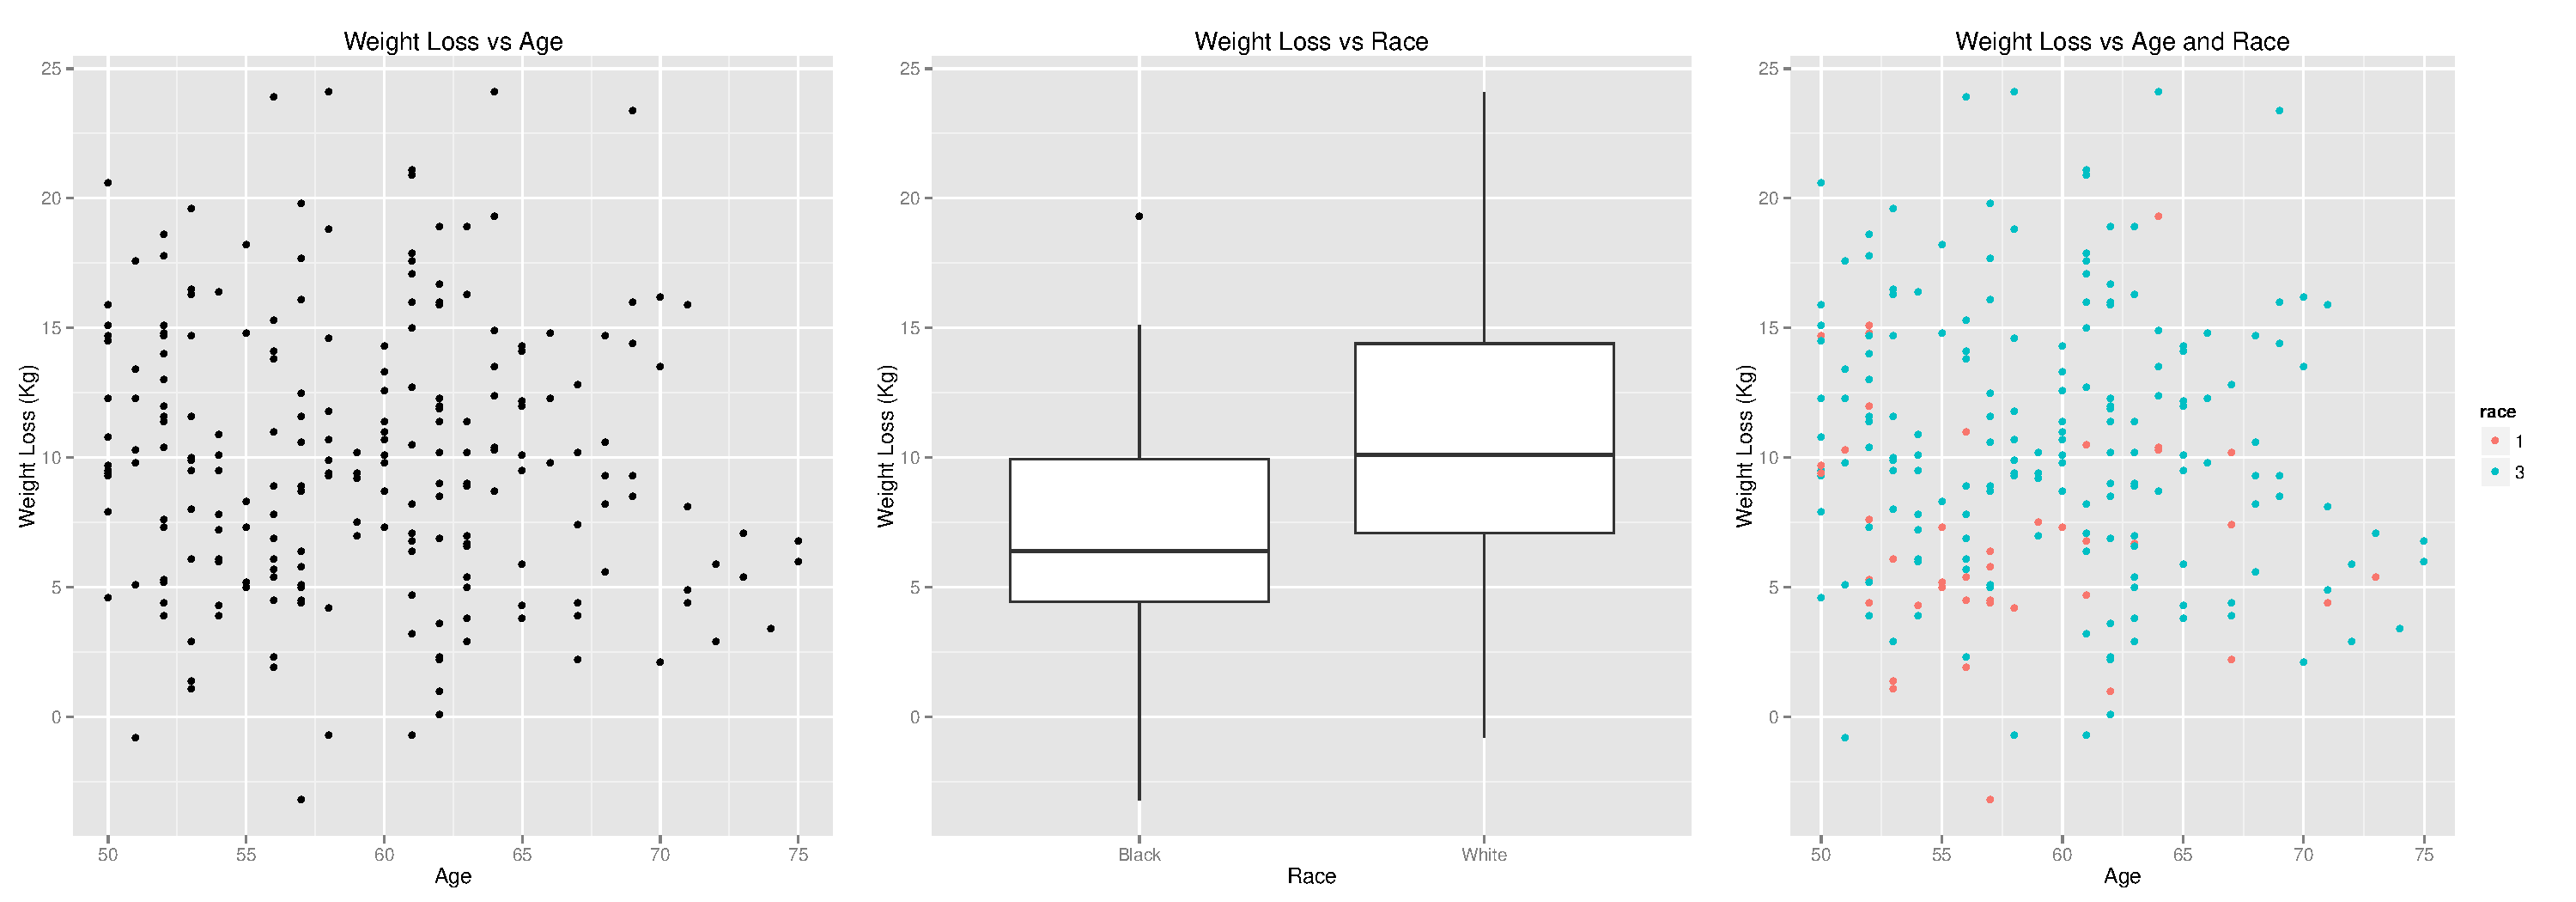
\includegraphics[scale = 0.4]{../image/weight-age-race}}
  \caption[]{\label{ch2:fig:tours} Scatterplots of weight loss vs age and
    Boxplots of weight loss for each race.  The boxplots use the
    default settings: (0.75, 0.5, 0.25) quantile for box and
    $Q1-1.5IQR$ for lower whisker and $Q3+1.5IQR$ for upper whisker. }
\end{figure}

\begin{table}[h]
  \caption[]{\label{ch2:tab:tours} 95\% credible (confidence) intervals for
    quantile regression parameters for TOURS. RQ is  the
    traditional frequentist approach using the quantreg package \citep{quantreg}, FBQR, method introduced in \cite{reich2010},
    PT, our proposed \polya{} trees approach with normal priors, and PTSS,
    \polya{} trees approach with spike-slab priors .}
  \vspace{4mm}

  \centering
  \begin{tabular}[tb]{l|l|l|l|l}
    \toprule
    Term      & PT                 & PTSS               & RQ                 & FBQR               \\
    \hline
    10\%      &                    &                    &                    &                    \\
    Intercept & 2.62(1.11,4.22)    & 2.10(0.65,3.36)    & 2.20(1.39,4.63)    & 1.90(0.04,3.62)    \\
    Age       & -0.57(-1.25,-0.03) & -0.57(-1.09,-0.07) & -0.25(-0.73,0.16)  & -0.32(-0.99,0.36)  \\
    Race      & 2.70(1.20,4.29)    & 3.32(2.07,4.70)    & 2.40(-0.23,3.92)   & 2.92(0.91,5.06)    \\
    \hline
    30\%      &                    &                    &                    &                    \\
    Intercept & 5.59(4.64,6.70)    & 5.45(4.41,6.36)    & 5.56(4.83,6.52)    & 5.32(3.67,6.80)    \\
    Age       & -0.46(-0.91,-0.10) & -0.47(-0.82,-0.19) & -0.66(-1.28,0.05)  & -0.47(-1.02,0.05)  \\
    Race      & 3.38(2.22,4.42)    & 3.58(2.56,4.65)    & 3.74(2.04,4.42)    & 3.56(1.99,5.20)    \\
    \hline
    50\%      &                    &                    &                    &                    \\
    Intercept & 7.43(6.46,8.56)    & 7.47(6.24,8.40)    & 7.83(5.42,9.09)    & 7.55(6.07,9.13)    \\
    Age       & -0.40(-0.75,-0.08) & -0.42(-0.72,-0.16) & -0.57(-1.04,0.14)  & -0.50(-1.06,0.03)  \\
    Race      & 3.81(2.77,4.68)    & 3.74(2.76,4.72)    & 3.53(2.52,5.46)    & 3.89(2.36,5.33)    \\
    \hline
    70\%      &                    &                    &                    &                    \\
    Intercept & 9.79(8.74,11.09)   & 10.12(8.92,11.18)  & 9.70(7.95,12.39)   & 9.84(8.11,11.83)   \\
    Age       & -0.31(-0.74,0.06)  & -0.34(-0.74,0.00)  & -0.69(-1.12,0.20)  & -0.57(-1.16,0.04)  \\
    Race      & 4.35(3.19,5.39)    & 3.94(2.87,4.99)    & 4.80(2.11,6.61)    & 4.30(2.59,5.75)    \\
    \hline
    90\%      &                    &                    &                    &                    \\
    Intercept & 12.80(11.30,14.62) & 13.53(11.98,15.06) & 12.61(11.48,15.27) & 13.65(11.65,15.86) \\
    Age       & -0.20(-0.89,0.38)  & -0.24(-0.86,0.30)  & -0.71(-1.59,-0.05) & -0.55(-1.38,0.42)  \\
    Race      & 5.05(3.36,6.61)    & 4.21(2.85,5.51)    & 6.08(2.48,6.85)    & 4.69(2.39,6.86)    \\
    \bottomrule
  \end{tabular}
\end{table}

Results appear in Table~\ref{ch2:tab:tours}.  Whites lost more weight than
blacks for all quantiles.  The differential is reported as significant
by PT and PTSS, and becomes larger when comparing more successful
weight losers (70\% - 90\% percentile). For example, whites lost 5.05
kg more than blacks among people losing the most weight (90\%)
reported from method PT (4.21 kg from PTSS).

The effect of age on the weight loss is small and not significant in
most cases (only barely significant in 10\% and 30\% quantile
regression by PT and PTSS).  The trend is negative showing that older
people tend to lose less weight. For example, median weight loss is
0.40 kg less for every age increase of 5 years reported by PT.

PTSS tends to shrink coefficients toward zero. For example, the
posterior probability that the heterogeneity parameters are zero are
all 100\% for Age and 99\% for Race, indicating there is no
heterogeneity for covariates AGE and RACE. This can help to select
variables in Bayesian models. For example, we can exclude AGE out of
the regressors or conclude the variance is homogeneous on the AGE
covariate.

\subsection{Comparison to FBQR and RQ}

Results from method RQ and FBQR show similar conclusions as PT and
PTSS.  But there are still differences on the estimates and
statistical significance.

For 10\% quantile, RQ reports Race is not an significant factor, which
differs from the other three methods.

For 30\% quantile, Age is not significant factor on weight loss from
RQ and FBQR. However, both PT and PTSS report Age has a significant
negative effect.

For 50\% and 70\% quantile, the four methods have some differences on
the estimates, but they all have agreements on the significances of
the covariates.

For 90\% quantile, RQ method provides different results than
others. Age is reported as significant on weight loss, while the other
methods show Age does not affect the 90\% quantile for weight loss.

\section{Discussion}
\label{ch2:sec:discussion}
This paper introduced a Bayesian approach for simultaneous linear
quantile regression by introducing mixture of \polya{} tree priors and
estimating heterogeneity parameters. By marginalizing the predictive
density function of the \polya{} tree distribution, quantiles of
interest can be obtained in closed form by inverting the predictive
cumulative distribution. Exact posterior inference can be made via
MCMC. Here, quantile lines cannot cross since quantiles are estimated
through density estimation. The simulations show our method performs
better than the frequentist approach especially when the error is
multimodal and highly skewed.  We also applied and illustrated our
approach on the Tours data exploring the relationship between
quantiles of weight loss and age and race.

Further research includes quantile regression for correlated data by
modelling error as a mixture of multivariate \polya{} tree
distribution.  Our approach allows for quantile regression with
missing data under ignorability by adding a data augmentation step.
We are exploring extending our approach to allow for nonignorable
missingness. Also it might be possible to use a slightly more complex
baseline distribution in \polya{} tree adaptively to improve the
estimation.


\bibliographystyle{plainnat} \bibliography{qr-draft-reference}

\end{document}
%%% Local Variables:
%%% mode: latex
%%% TeX-master: t
%%% End:
